\scanpage{57}
\deleted{Fixons un $v$ de référence (i.e. une topologie sur $k$, \unsure{déterm.} \unsure{isom.} $k\simeq\mathbf C$ mod conj. compl.).}

Or $g_\sigma$ est connu mod mult. à droite par $G(\mathbf Z)$, d'autre part $g_{\sigma\,\mathrm{fini}}$ est (avec la $=$ indétermination) le système des $\sigma_\ell$ galoisiens. Donc on peut prendre
\[
g_\sigma=((\deleted{g_\ell}\inserted{\sigma_\ell})_{\ell\ \mathrm{fini}},\sigma_\infty)
\]
\uline{où maintenant} $\sigma_\infty$ \uline{est un élément bien déterminé de} $G(\unsure{k|K})$ !!!

On obtient une application canonique
\diagram{\begin{tikzcd}[ampersand replacement=\&,column sep=large,execute at end picture={\draw ([xshift=-7pt,yshift=13pt]current bounding box.north west) rectangle ([xshift=-72pt,yshift=-13pt]current bounding box.south east);}]
\operatorname{Gal}(k/k_0)\arrow[r,"\varphi_v"]\&G_{\deleted{\unsure{\xi_v}}}(\unsure{k|K})\subset\mathrm{Gl}(M_k(\infty))
\end{tikzcd}}
\margin{\figure{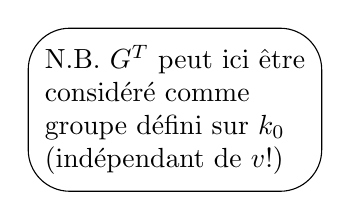
\begin{tikzpicture}\node[draw,rounded corners=15pt,align=left,inner sep=6pt] {N.B. $G^T$ peut ici être\\considéré comme\\groupe défini sur $k_0$\\(\uline{indépendant de $v$!})};\end{tikzpicture}}}
et telle qu'on ait
\diagram{\begin{tikzcd}[ampersand replacement=\&,column sep=small]
\dot\sigma M_v^{\mathbf Z}\arrow[r,equal]\&\left\{\begin{array}{l}M_{\sigma v}^{\mathbf Z}=\sigma_*M_v^{\mathbf Z}\qquad\text{pour }\sigma\in\operatorname{Gal}(k/k_0)\\[7pt]\sigma_*=((\sigma_\ell)_{\ell\ \mathrm{fini}},\varphi_v(\sigma)).\end{array}\right.
\end{tikzcd}}

On vérifie aussitôt
\[
\varphi_v(\tau\sigma)={}^\tau\varphi_v(\sigma)^{\deleted{\unsure{\tau|-1}}}\varphi_v(\tau)
\]
i.e. posant $\psi_v=\varphi_v^{-1}$
\[
\psi_v(\tau\sigma)=\psi_v(\tau){}^\tau\psi_v(\sigma)^{\deleted{\unsure{\tau|-1}}}
\]
\mspage{56}
